\documentclass[8pt,aspectratio=169,hyperref={unicode=true}]{beamer}

\usefonttheme{serif}
\usepackage{fontspec}
	\setmainfont{TeX Gyre Heros}
\usepackage{unicode-math}
\usepackage{lualatex-math}
	\setmathfont{TeX Gyre Termes Math}
\usepackage{polyglossia}
\setdefaultlanguage[frenchpart=false]{french}
\setotherlanguage{english}
%\usepackage{microtype}
\usepackage[locale = FR,
            separate-uncertainty,
            multi-part-units = single,
            range-units = single]{siunitx}
	\DeclareSIUnit\an{an}
  \DeclareSIUnit{\octet}{o}
\usepackage{amsmath}
\usepackage{amsfonts}
\usepackage{amssymb}
\usepackage{array}
\usepackage{graphicx}
\graphicspath{{./Figures/}}
\usepackage{booktabs}
\usepackage{tabularx}
\usepackage{multirow}
\usepackage{multicol}
    \newcolumntype{L}{>{\raggedright\arraybackslash}X}
    \newcolumntype{R}{>{\raggedleft\arraybackslash}X}
\usepackage{makecell}
\setcellgapes{5pt}
\usepackage{xcolor}
\usepackage{tikz}
\usetikzlibrary{graphs, graphdrawing, arrows.meta} \usegdlibrary{layered, trees}
\usetikzlibrary{overlay-beamer-styles}
\usepackage{subcaption}
\usepackage[]{animate}
\usepackage{float}
\usepackage{csquotes}
\usepackage{minted}
\usepackage{xurl}

\usetheme[secheader]{Boadilla}
\usecolortheme{seagull}
\setbeamertemplate{enumerate items}[default]
\setbeamertemplate{itemize items}{-}
\setbeamertemplate{navigation symbols}{}
\setbeamertemplate{bibliography item}{}
\setbeamerfont{framesubtitle}{size=\large}
\setbeamertemplate{section in toc}[sections numbered]
%\setbeamertemplate{subsection in toc}[subsections numbered]

\title[Déployez un modèle dans le cloud]{Projet 8 : Déployez un modèle dans le cloud}
\author[Lancelot \textsc{Leclercq}]{Lancelot \textsc{Leclercq}} 
\institute[]{}
\date[]{\small{10 juin 2022}}

\AtBeginSection[]{
  \begin{frame}
  \vfill
  \centering
    \usebeamerfont{title}\insertsectionhead\par%
  \vfill
  \end{frame}
}

\begin{document}
\setbeamercolor{background canvas}{bg=gray!20}
\begin{frame}[plain]
  \titlepage
\end{frame}

\begin{frame}{Sommaire}
  \Large
  \begin{columns}
    \begin{column}{.7\textwidth}
      \tableofcontents[hideallsubsections]
    \end{column}
  \end{columns}
\end{frame}

\section{Introduction}
\subsection{Problématique}
\begin{frame}{\insertsubsection}
  \begin{columns}
    \begin{column}{.6\textwidth}
      \begin{itemize}
        \item Préservation de la biodiversité des fruits
              \begin{itemize}
                \item traitements spécifiques pour chaque espèce de fruits par des robots cueilleurs intelligents
              \end{itemize}
        \item[]
        \item 1ère étape développer une application mobile
              \begin{itemize}
                \item Permettre à l'utilisateur d'obtenir des informations sur un fruit à partir d'une photo
                \item[]
                \item Sensibiliser le grand public à la biodiversité des fruits
                \item[]
                \item Mettre en place une première version du moteur de classification des images de fruits
                \item[]
                \item Construire une première version de l'architecture Big Data
              \end{itemize}
      \end{itemize}

    \end{column}
    \begin{column}{.4\textwidth}
      \center
      
\includegraphics[width=\textwidth]{./Logo projet big data.png}
    \end{column}
  \end{columns}
\end{frame}

\subsection{Données}
\begin{frame}{\insertsubsection}
  \begin{columns}
    \begin{column}{.6\textwidth}
      \begin{itemize}
        \item Utilisation du jeu de données Kaggle : \url{https://www.kaggle.com/datasets/moltean/fruits}
        \item[]
        \item Nombre total d'images : 90483
        \item[]
        \item Taille du jeu d'entrainement : 67692 images
        \item[]
        \item Taille du jeu de test : 22688 images
        \item[]
        \item  Nombre de fruits : 131
      \end{itemize}
    \end{column}
    \begin{column}{.4\textwidth}
      \begin{itemize}
        \item Exemple d'image de fruit :
        \item[]
      \end{itemize}
      \center
      \includegraphics[width=.8\textwidth]{./fruits-360_dataset/fruits-360/Training/Strawberry/0_100.jpg}
    \end{column}
  \end{columns}
\end{frame}

\section{BigData}
\subsection{Spark}
\begin{frame}{\insertsubsection}
  \begin{columns}
    \begin{column}{.6\textwidth}
      \begin{itemize}
        \item Parallélisation des calculs
              \begin{itemize}
                \item Utilisation de plusieurs machines
                \item[]
                \item Distribution des calculs
              \end{itemize}
        \item[]
        \item Coût d'utilisation des machines à surveiller
        \item[]
        \item Utilisation de PySpark une interface Spark en python
      \end{itemize}
    \end{column}
    \begin{column}{.4\textwidth}
      
\includegraphics[width=\textwidth]{./spark.pdf}
    \end{column}
  \end{columns}
  \vfill
  \begin{center}
    \tikz [rounded corners, every node/.style={anchor=west}, level sep = 4mm, >={Stealth}]
    \graph [layered layout, grow=right, nodes={draw, font=\footnotesize}, head anchor=west, tail anchor=east,
    edges=rounded corners, sibling distance=5mm]{
    Importation images ->  Détection -> "Clusterisation (1000 groupes de descripteurs)" -> "PCA (conservation de 100 composantes)" -> "création fichier .csv",
    "Détection des descripteurs (OpenCV)" [draw] // {Détection, "Clusterisation (1000 groupes de descripteurs)"},
    "Réduction de dimension"  [draw]  // {"PCA (conservation de 100 composantes)"},
    };
  \end{center}
\end{frame}

\begin{frame}{\insertsubsection}
  \begin{columns}
    \begin{column}{.5\textwidth}
      \begin{itemize}
        \item SparkContext supervise la répartition des taches
        \item[]
        \item Différentes taches sont réparties sur les différents nœuds
      \end{itemize}
    \end{column}
    \begin{column}{.5\textwidth}
      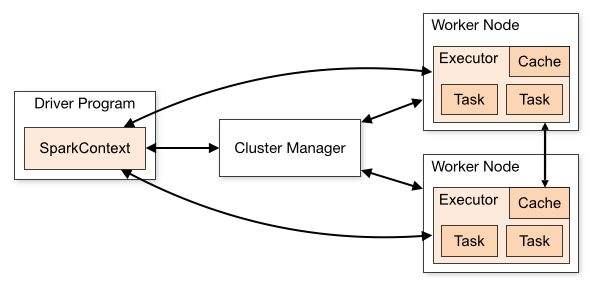
\includegraphics[width=\textwidth]{./cluster-overview.png}
    \end{column}
  \end{columns}
\end{frame}

\subsection{PySpark}
\subsubsection{Importation des données}
\begin{frame}[fragile]{\insertsubsection : \insertsubsubsection}
  \begin{columns}
    \begin{column}{.25\textwidth}
      \begin{itemize}
        \item Importation des images au format binaire :
      \end{itemize}
    \end{column}
    \begin{column}{.75\textwidth}
      \begin{minted}{python}
ImgData = spark.read.format('binaryFile') \
                  .option('pathGlobFilter', '*.jpg') \
                  .option('recursiveFileLookup', 'true') \
                  .load(path) \
                  .select('path', 'content')   
      \end{minted}
    \end{column}
  \end{columns}

  \vfill
  \hrule

  \begin{columns}
    \begin{column}{.25\textwidth}
      \begin{itemize}
        \item Récupération d'un label (nom du fruit et espèce) à partir du chemin d'accès au fichier image :
      \end{itemize}
    \end{column}
    \begin{column}{.75\textwidth}
      \begin{minted}{python}
ImgData = ImgData.withColumn('label',
                             F.element_at(F.split(F.col('path'), '/'), -2))
      \end{minted}
    \end{column}
  \end{columns}

  \vfill
  \hrule

  \begin{columns}
    \begin{column}{.25\textwidth}
      \begin{itemize}
        \item Création d'un nom d'image du label et du nom de l'image :
        \item Ex :
              \begin{itemize}
                \item image : 0\_100.jpg
                \item label : Apricot
                \item nom : Apricot\_0\_100.jpg
              \end{itemize}
      \end{itemize}
    \end{column}
    \begin{column}{.75\textwidth}
      \begin{minted}{python}
ImgData = ImgData.withColumn(
    'imgName',
    F.concat('label', F.lit('_'), F.element_at(F.split(F.col('path'), '/'),
                                               -1)))
      \end{minted}
    \end{column}
  \end{columns}
\end{frame}

\subsubsection{Détection des descripteurs}
\begin{frame}[fragile]{\insertsubsection : \insertsubsubsection}
  \begin{columns}
    \begin{column}{.3\textwidth}
      \begin{itemize}
        \item Fonction permettant de détecter les descripteurs avec OpenCV :
        \item[]
        \item Utilisation des données binaires des images grâce à io.BytesIO
        \item[]
        \item Inspiré de \url{https://stackoverflow.com/questions/60192589/problem-with-pyspark-udf-to-get-descriptors-with-opencv-problem}
      \end{itemize}
    \end{column}
    \begin{column}{.7\textwidth}
      \begin{minted}{python}
def get_desc(content):
    try:
        img = np.array(Image.open(io.BytesIO(content)))
    except:
        print(content)
        img = None
        return img
    if img is None:
        desc = None
    else:
        orb = cv.ORB_create(nfeatures=100)
        keypoints_orb, desc = orb.detectAndCompute(img, None)
    if desc is None:
        desc = [np.array(32 * [0]).astype(np.float64).tolist()]
    else:
        desc = desc.astype(np.float64).tolist()
    return desc
      \end{minted}
    \end{column}
  \end{columns}
  \vspace{3px}
  \hrule
  \begin{columns}
    \begin{column}{.25\textwidth}
      \begin{itemize}
        \item Création d'une colonne avec les descripteurs détectés pas OpenCV :
      \end{itemize}
    \end{column}
    \begin{column}{.75\textwidth}
      \begin{minted}{python}
udf_image = F.udf(
    get_desc,
    ArrayType(ArrayType(FloatType(), containsNull=False), containsNull=False))
ImgDesc = ImgData.withColumn("descriptors", F.explode(udf_image("content")))  
      \end{minted}
    \end{column}
  \end{columns}
\end{frame}

\subsubsection{Création d'un \emph{bag of visual words}}
\begin{frame}[fragile]{\insertsubsection : \insertsubsubsection}
  \begin{columns}
    \begin{column}{.3\textwidth}
      \begin{itemize}
        \item Utilisation des fonction de machine learning de pyspark : KMeans
              \begin{itemize}
                \item Création de groupes de descripteurs
              \end{itemize}
      \end{itemize}
    \end{column}
    \begin{column}{.7\textwidth}
      \begin{minted}{python}
kmean = KMeans(k=1000, featuresCol='descriptors', seed=0)
model = kmean.fit(ImgDesc)

Pred = model.transform(ImgDesc)
      \end{minted}
    \end{column}
  \end{columns}

  \vfill
  \hrule

  \begin{columns}
    \begin{column}{.25\textwidth}
      \begin{itemize}
        \item Utilisation de la fonction groupBy pour compter le nombre d'occurrences de chaques groupes de descripteurs
      \end{itemize}
    \end{column}
    \begin{column}{.75\textwidth}
      \begin{minted}{python}
ImgPred = Pred.groupBy('label', 'prediction').count()

BoVW = ImgPred.groupBy('label').pivot('prediction').sum('count').fillna(0)
      \end{minted}
    \end{column}
  \end{columns}
\end{frame}

\subsubsection{Réduction de dimension}
\begin{frame}[fragile]{\insertsubsection : \insertsubsubsection}
  \begin{columns}
    \begin{column}{.25\textwidth}
      \begin{itemize}
        \item Réduction de dimension par PCA :
      \end{itemize}
    \end{column}
    \begin{column}{.75\textwidth}
      \begin{minted}{python}
VA = VectorAssembler(inputCols=BoVW.drop('label').columns,
                     outputCol='features')
pca = PCA(k=100, inputCol='features', outputCol='pca_features')
pipe = Pipeline(stages=[VA, pca])

pipePCA = pipe.fit(BoVW)

pcaData = pipePCA.transform(BoVW)
pcaDataDF = pcaData.select(['label', 'pca_features']).toPandas()
      \end{minted}
    \end{column}
  \end{columns}
\end{frame}

\section{Déploiement sur le cloud}
\begin{frame}{\insertsection}
  \begin{columns}
    \begin{column}{.6\textwidth}
      \begin{itemize}
        \item Utilisation d'une machine EC2 hébergée par Amazon Web Services
              \begin{itemize}
                \item Utilisation de Debian
                \item[]
                \item Connexion par SSH
                \item[]
                \item Installation de java, git
              \end{itemize}
        \item[]
        \item Utilisation de S3 comme espace de stockage pour la base de données d'images
      \end{itemize}
    \end{column}
    \begin{column}{.4\textwidth}
      \center
      
\includegraphics[width=.8\textwidth]{./512px-Amazon_Web_Services_Logo.svg.png}
    \end{column}
  \end{columns}
\end{frame}

\begin{frame}{\insertsection}
  \begin{columns}
    \begin{column}{.5\textwidth}
      \begin{itemize}
        \item Essais avec t2.micro
              \begin{itemize}
                \item 1 CPU
                \item \SI{1}{\giga\byte} de mémoire RAM
                \item \SI{10}{\giga\octet} de mémoire disque
                \item Connexion réseau lente
              \end{itemize}
        \item[]
        \item Utilisation d'un jeu d'entrainement très léger : 2 types de fruits
        \item[]
        \item Offre gratuite
        \item[]
        \item Coût très faible, mais peu de ressources de calculs
      \end{itemize}
    \end{column}
    \begin{column}{.5\textwidth}
      \begin{itemize}
        \item Essais avec t3.2xlarge
              \begin{itemize}
                \item 8 CPU
                \item \SI{32}{\giga\byte} de mémoire RAM
                \item \SI{10}{\giga\octet} de mémoire disque
                \item Connexion réseau jusqu'à \SI{5}{\giga\bit}
              \end{itemize}
        \item[]
        \item Sample d'un dixième de la base originale $\simeq$ 60000 image soit environ 6000 images
        \item[]
        \item \SI{0.3776}{\$} par heure
        \item[]
        \item Coût plus important, mais supporte mieux la charge de calculs
      \end{itemize}
    \end{column}
  \end{columns}
\end{frame}

\subsection{Configuration de l'utilisation des services Amazon}
\begin{frame}[fragile]{\insertsection}{\insertsubsection}
  \begin{itemize}
    \item Téléchargement des packages permettant de communiquer avec le stockage S3
  \end{itemize}
  \begin{minted}{python}
os.environ[
    'PYSPARK_SUBMIT_ARGS'] = '--packages com.amazonaws:aws-java-sdk:1.12.230, \
                                org.apache.hadoop:hadoop-aws:3.3.1 pyspark-shell'
  \end{minted}

  \vfill
  \hrule

  \begin{itemize}
    \item Configuration de hadoop pour gérer la connexion au stockage sur S3
    \begin{itemize}
      \item Utilisation d'un fichier \emph{credentials} dans le dossier ~/.aws/ afin d'avoir les clés de connexion facilement accessibles
    \end{itemize}
  \end{itemize}
  \begin{minted}{python}
  spark = SparkSession.builder.master('local').appName(
      'FruitsPreProc').getOrCreate()
  sc = spark.sparkContext
  sc._jsc.hadoopConfiguration().set('fs.s3a.impl',
                                    'org.apache.hadoop.fs.s3a.S3AFileSystem')
  sc._jsc.hadoopConfiguration().set(
      "fs.s3a.aws.credentials.provider",
      "com.amazonaws.auth.profile.ProfileCredentialsProvider")
  sc._jsc.hadoopConfiguration().set("fs.s3a.endpoint",
                                    "s3.eu-west-3.amazonaws.com")
  spark.sparkContext._conf.getAll()
    \end{minted}
\end{frame}

\section{Axes d'amélioration}
\begin{frame}{\insertsection}
  \begin{itemize}
    \item KMeans instable, difficile à débugger :
    \item[$\Rightarrow$] Essayer d'autres alternatives comme dask
    \item[]
    \item Utilisation d'un EMR permettant d'avoir les calculs réalisés par plusieurs machines
    \item[]
    \item Ajout d'un modèle de classification afin de classer les fruits
    \item[]
    \item Affiner les catégories avec des maturités différentes afin de cueillir les fruits au meilleur moment
  \end{itemize}
\end{frame}
\end{document}


